\begin{frame}{Cross-Validation}{k-Fold cross-validation}

\begin{enumerate}
    \item Randomly divide the set of observations into $k$ groups, or folds, of approximately equal size.  \pause 
    
    \item The first fold is treated as a validation set, and the method is fit on the remaining $k - 1$ folds.  \pause 
    
    \item The mean squared error, $MSE_1$ , is then computed on the observations in the held-out fold.  \pause 
    
    \item Repeated this procedure $k$ times; each time. \\ \pause 
    $\rightarrow$ A different group of observations is treated as a validation set. \\ \pause
    $\rightarrow$ This process results in $k$ estimates of the test error, $MSE_1 , MSE_2 , \cdots , MSE_k$.  \pause 
    
    \item The k-fold CV estimate is computed by averaging these values.

    \begin{equation}
        CV_{(k)} = \frac{1}{k} \sum_{i=1}^k MSE_i. 
    \end{equation}
\end{enumerate}
    
\end{frame}

\begin{frame}{Cross-Validation}{k-Fold Cross-Validation}

\begin{figure}
    \centering
    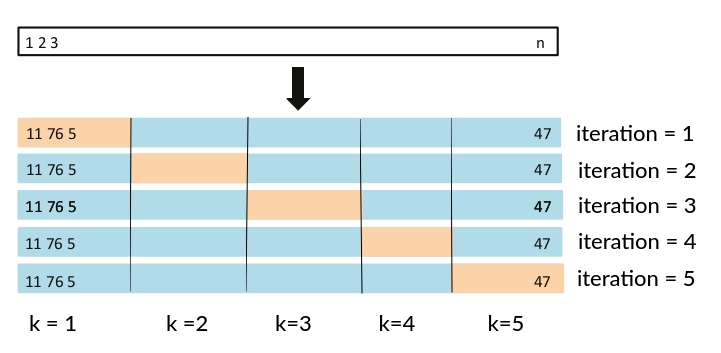
\includegraphics[height=4cm]{cross-val/kfold.png}
\end{figure} \pause 


\begin{itemize}
    \item LOOCV is a special case of k-fold CV in which $k$
is set to equal $n$. \pause 
    \item In practice, one typically performs k-fold CV using $k = 5$ or $k = 10$. \pause 
    \item What is the advantage of using $k = 5$ or $k = 10$ rather than $k = n$? \pause \\
    $\rightarrow$ The most obvious advantage is computational. 
    
\end{itemize}
    
\end{frame}
